
\noindent\begin{tabular}{@{}p{0.285\linewidth}p{0.37\linewidth}p{0.285\linewidth}@{}}
\centering\textbf{Problem Chosen}\par\Large\Problem &
\centering\textbf{Synthetic Rehearsal}\par\textbf{Summary Sheet} &
\centering\textbf{Team Control Number}\par\Large\Team\tabularnewline
\end{tabular}
\par\vspace{0.8em}\hrule\vspace{1em}
\begin{center}
{\Large\bfseries Synthetic Presentation Rehearsal}\end{center}
This document tests a shared manuscript layout and a bounded figure repair loop.
All curves, surfaces and trajectories are synthetic demonstrations. They do not
describe a real competition solution, field observation or approved result.
The comparison uses identical source figures before and after a single width edit.
The original manuscript and project registries must remain unchanged.
\par\textbf{Keywords:} synthetic example; scientific figures; reproducible layout.

\clearpage
\section{Layout and Figure Verification}
This short synthetic specimen tests the shared font and layout defaults. It is
not a complete modeling paper. Figure~\ref{fig:width} starts wider than the text
column to exercise a bounded repair. The plotted values must remain unchanged.
\begin{figure}[htbp]
\centering
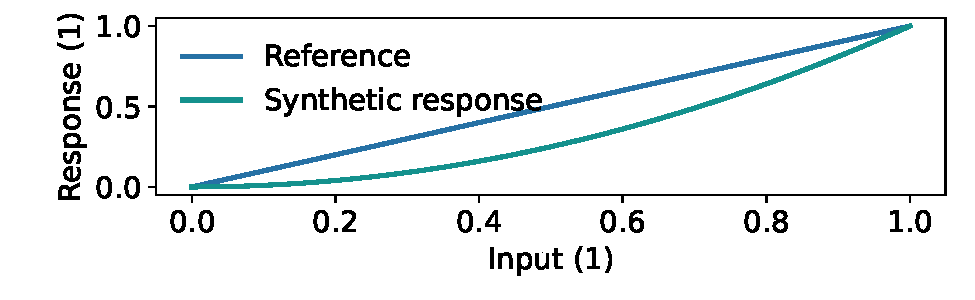
\includegraphics[width=\linewidth]{width-demo.pdf}
\caption{Fixed synthetic curves. The axes use dimensionless units.}
\label{fig:width}
\end{figure}
\subsection{Three dimensions with direct readout}
Figure~\ref{fig:surface} combines a response surface with the same grid in plan
view. Figure~\ref{fig:trajectory} uses true spatial coordinates with XY and XZ
projections. Their data, units, color ranges and source hashes are fixed.
Neither demonstration establishes a real mechanism or an optimal decision.
\subsection{Checks and interpretation}
Compilation, pixel-complete page rendering and font checks are separate from
visual acceptance. A source-label crop and an interior blank area were found
in an earlier specimen and corrected before this version. The repair loop
changes only a supported insertion width; complex layouts remain review tasks.
\begin{thebibliography}{1}
\bibitem{recipe} Self-authored synthetic scientific-figure recipes (2026).
\end{thebibliography}
\section*{Report on Use of AI Tools}
Codex generated the specimen and plotting code. Fixed-version build, fault and
non-author review records describe their actual scope; no user approval is implied.
\clearpage
\begin{figure}[p]
\centering
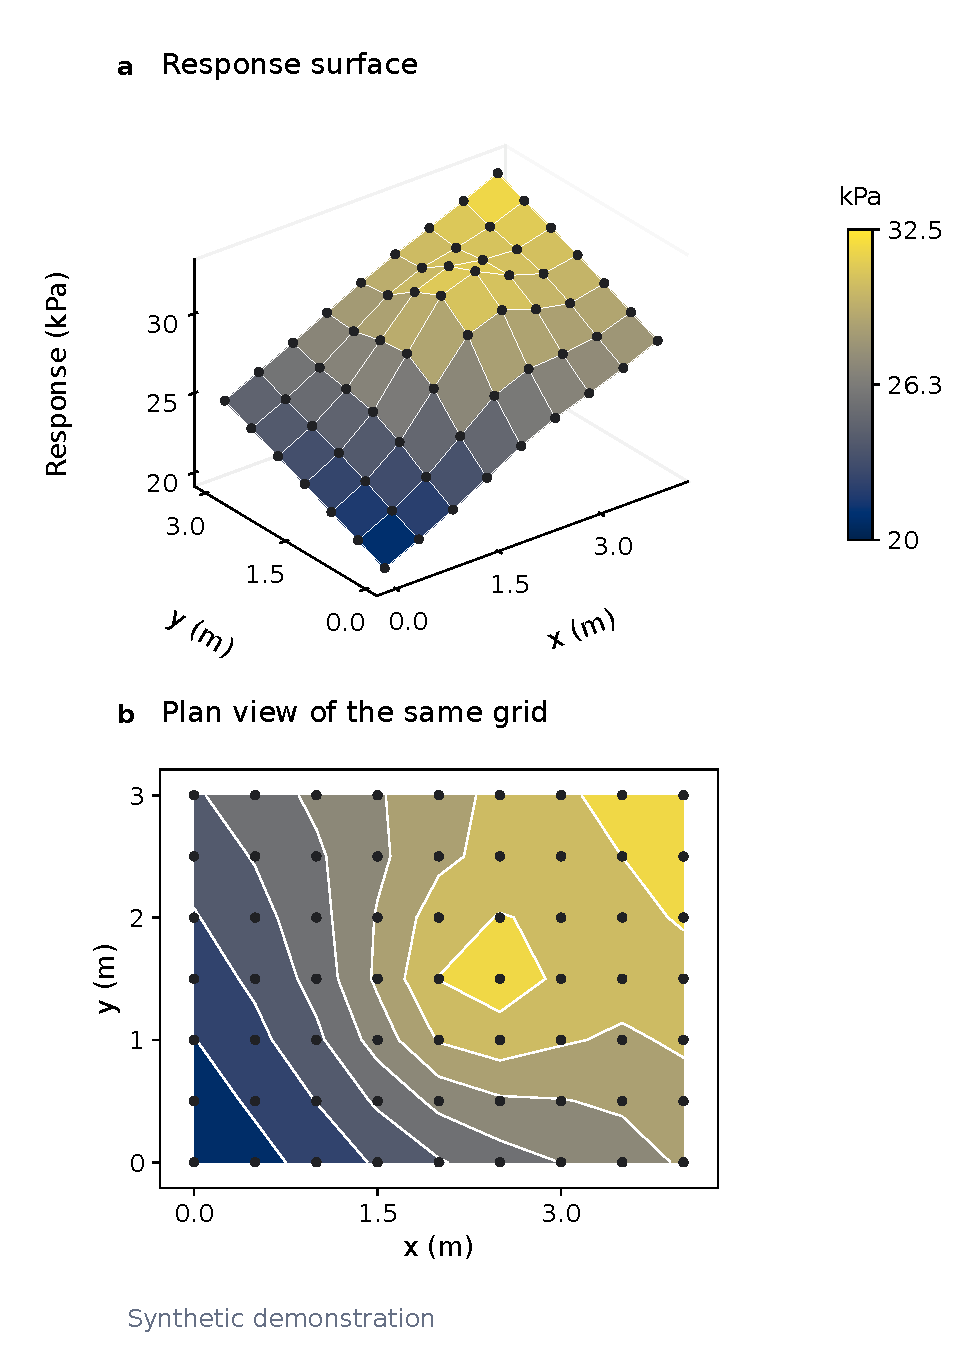
\includegraphics[width=\linewidth]{surface.pdf}
\caption{Synthetic response surface and same-data contour companion.}
\label{fig:surface}
\end{figure}
\clearpage
\begin{figure}[p]
\centering
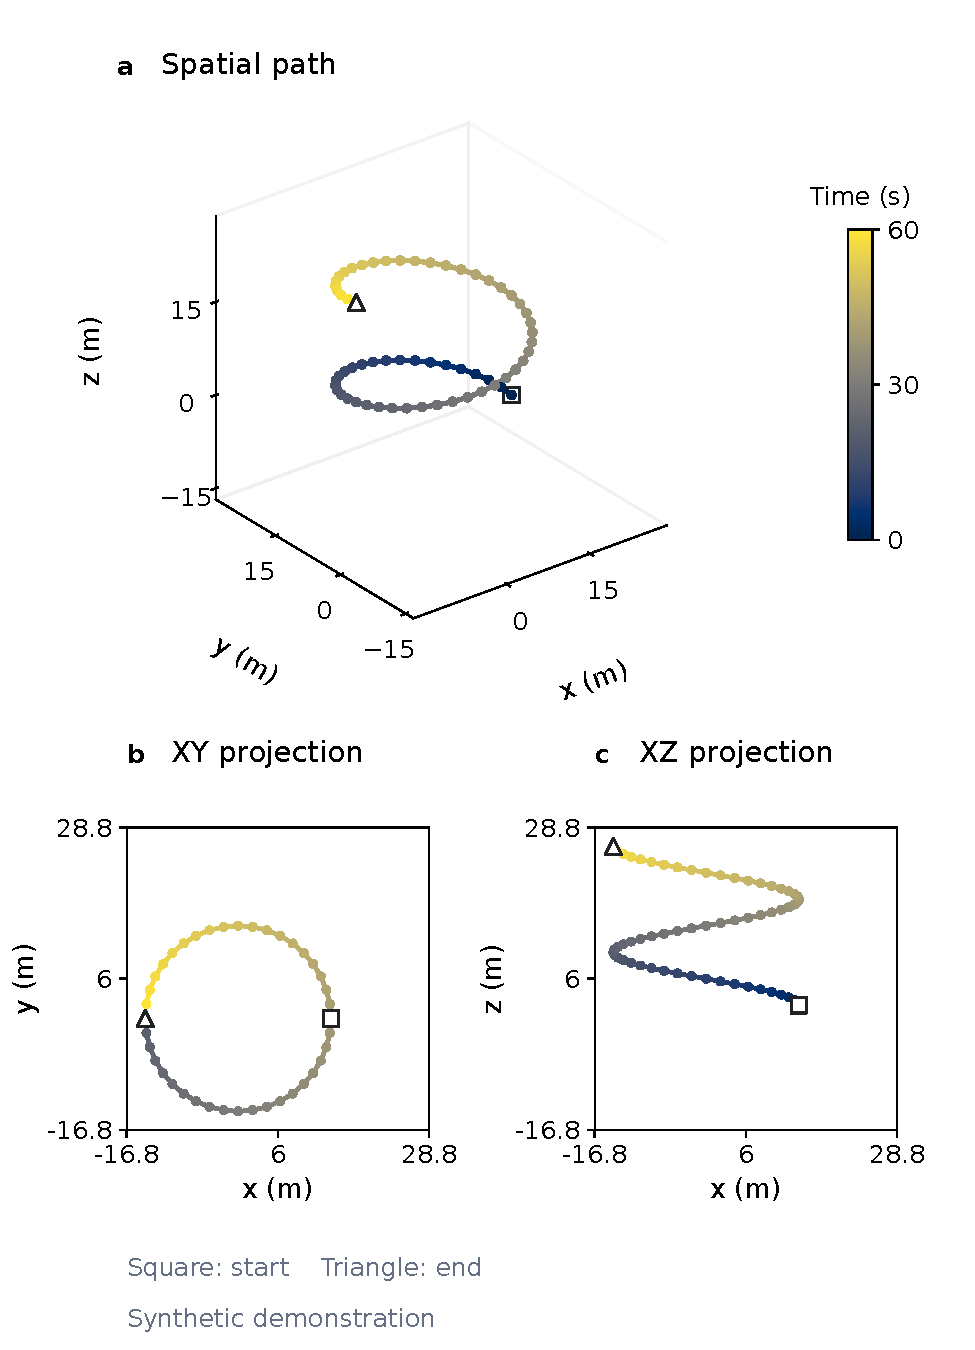
\includegraphics[width=\linewidth]{trajectory.pdf}
\caption{Synthetic spatial path with XY and XZ projections for direct reading.}
\label{fig:trajectory}
\label{main-report-end}
\end{figure}
\clearpage

